
\documentclass[12pt]{article}
\usepackage{geometry} % see geometry.pdf on how to lay out the page. There's lots.
\usepackage{hyperref}
\usepackage{url}
\usepackage{tikz}
\usetikzlibrary{arrows,automata}
\usepackage{amsmath}
\usepackage{ dsfont }
\geometry{a4paper} % or letter or a5paper or ... etc

\title{Data driven section}
\author{}
\date{} % delete this line to display the current date

\begin{document}
\maketitle

\section{Overview}
This section of the conversational model is meant to retrieve information on current events and interests in such a way as to be most relevant to the current conversation as possible. The model makes use of recent advances in Neural Network memory systems and well as topic classification.

\section{Architecture}
The architecture of the Data Driven (DD) section of the conversational system is given by figure~\ref{DD_design}. The topic nodes represent Dynamic Memory Networks (DMNs \cite{Kumar:2015ys}), and the TC node is a topic classifier to dispatch commands to one of the provided topics. 

\subsection{Data flow}
Plain english is passed into the Topic Classifier to determine which of the DMNs is most well suited to answer any questions posed, or provide relevant information. Then the english sentence is provided to the relevant DMN whose episodic memory design allows to it retrieve relevant recent events (see information gathering section~\ref{section_info}). This response is returned to the CC module for further processing and formatting.

\subsection{Topics}
The Topic DMNs can be separated into two groups: Global modules and User modules. 

\noindent
Global modules are populated with information deemed relevant to all users' interests, such as sports, politics, and culture. These modules can be queried by any DD module for any user and the same responses should be expected (i.e. ``Who won the game on Saturday'' is not user-dependent). As such these modules can be shared among all instances of the DD module.

\noindent
User modules are tailored to a specific user's interests. The TC module can double as a simple unsupervised learning system as well as a labeled topic classifier in order to determine what topics a specific user may find interesting. These topics can then be researched and added to the list of available topic DMNs.

\begin{figure}
    \centering
    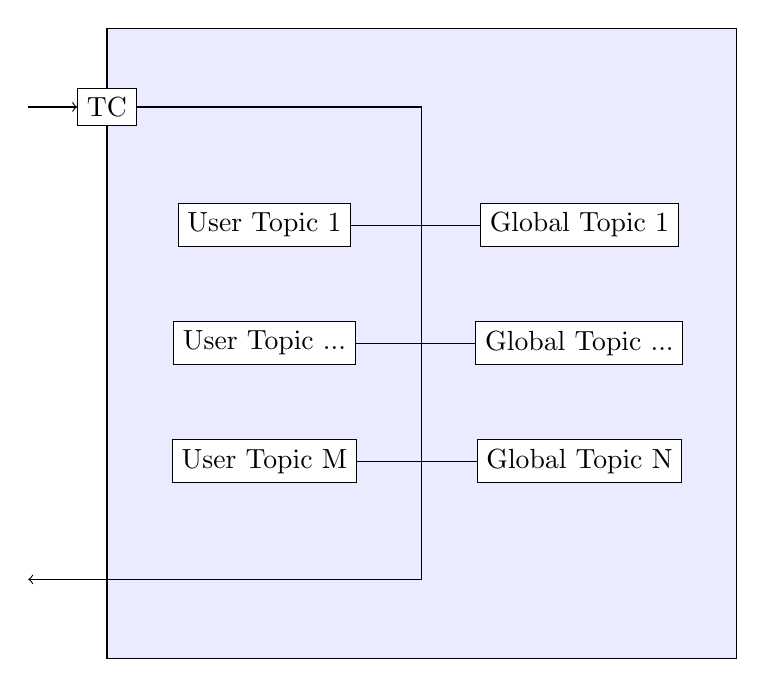
\begin{tikzpicture}
    	\tikzstyle{every node} = [draw,shape=rectangle,fill=white]
	\filldraw[fill=blue!40!white, draw=black, opacity=0.2] (1,0) rectangle (9,8);
	\draw (1,0) rectangle (9,8);
	
	\node (TC) at (1,7) {TC};
	
	\node (Topic1) at (7,5.5) {Global  Topic 1};
	\node (TopicE) at (7,4) {Global Topic ...};
	\node (TopicN) at (7,2.5) {Global Topic N};
	
	\node (UTopic1) at (3,5.5) {User Topic 1};
	\node (UTopicE) at (3,4) {User Topic ...};
	\node (UTopic2) at (3,2.5) {User Topic M};
	
	\draw [->] (0,7) -- (TC);
	\draw (TC) -- (5,7); \draw (5,7) -- (5,1);
	\draw [->] (5,1) -- (0,1);
	\draw (Topic1) -- (5,5.5);
	\draw (TopicE) -- (5,4);
	\draw (TopicN) -- (5,2.5);
	\draw (UTopic1) -- (5,5.5);
	\draw (UTopicE) -- (5,4);
	\draw (UTopic2) -- (5,2.5);
	
    \end{tikzpicture}
    \label{DD_design}
    \caption{DD architecture}
\end{figure}

\section{Information Gathering \label{section_info}}
Populating the DMNs is a constant process. The general implementation will be to discover facts on a topic via predefined news sources (i.e. Google News) or databases (i.e. Wikipedia) and to convert any fact tables into simple sentences. This means that information such as the tuple \emph{(Country: United States, Capital: Washington D.C.)} should be entered into the DMN as \emph{``The capital of the United States is Washington D.C.''}. Global topics should be constantly querying for the most relevant information, weighted by importance and age. More important topics should remain in the DMN longer, and more recent topics should be included. Should a query not find results in the topic's DMN then more classical Information Retrieval algorithms can be employed to compute the result and populate a user DMN for later reference. User DMNs will have a twofold responsibility. They will cover topics not relevant to the general population or which are more specific than generally necessary.
These user topics can be populated during a conversation, but also when the user is not active. Using the preexisting TC module we can query incoming news or database entries for information deemed relevant and important and populate the appropriate DMN for later conversations. 

\bibliographystyle{plain}
\bibliography{bib} 


\end{document}